The on-chain subsystem is the ultimate source of truth for rollup state and security. Written in \textbf{Solidity} and deployed using Hardhat, these contracts enforce the validity of state transitions and encode the data availability rules that bind L2 execution to L1 settlement.

\subsubsection{Overview}

The on-chain architecture is centered around \texttt{ZKRollupBridge.sol}, which acts as the settlement hub for batch commitments. The contract is explicitly designed for experimentation and modular evolution: it accepts multiple verifier implementations and DA provider implementations, allowing the system to benchmark different configurations without requiring a full contract redesign. This modularity is aligned with the overall PoC goal of evaluating proving and DA trade-offs in a controlled manner.

\begin{figure}[htbp]
 \begin{adjustwidth}{0cm}{}
  \centering
  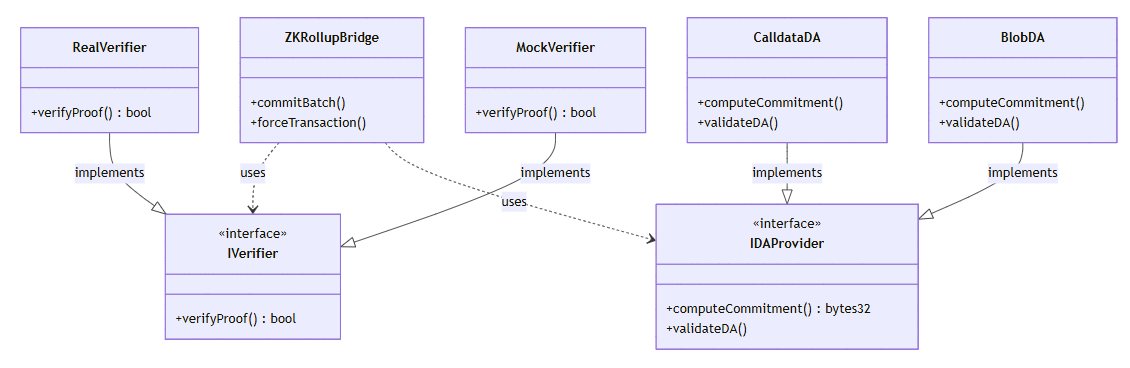
\includegraphics[width=0.95\linewidth]{figures/contract-interface.png}
  \caption{Contract Interface and Strategy Pattern.}
  \label{fig:contract-interface}
 \end{adjustwidth}
\end{figure}

\subsubsection{Architectural Components}

\subsubsubsection{ZKRollupBridge.sol}

\texttt{ZKRollupBridge.sol} is the primary entry point for settlement. It manages state root updates, validates submitted batch commitments, delegates proof verification to a verifier contract, and delegates DA validation to a DA provider contract.

A central design feature is the \textbf{Strategy Pattern} used to decouple the bridge from specific proof systems and DA mechanisms (Figure~\ref{fig:contract-interface}). The bridge maintains a mapping from \texttt{verifierId} to \texttt{IVerifier} implementations, allowing different verification behaviors to coexist under a unified interface. This makes it possible to use \texttt{verifierId=0} for real Groth16 verification on BN254, while reserving additional IDs for benchmarking-oriented verification paths for Plonky2 or Halo2.

\begin{lstlisting}[style=rustStyle, caption={Commit Batch with Modular Checks}, label={lst:commit-batch}]
function commitBatch(
    uint8 daId,
    uint8 verifierId,
    bytes calldata batchData,
    bytes calldata daMeta,
    bytes32 newRoot,
    bytes calldata proof
) external {
    _requireSequencer();

    // 1. Censorship Resistance Check
    if (forcedTxQueue.length > forcedHead) {
        // Ensure oldest forced tx hasn't expired
        // ...
    }

    // 2. Data Availability Validation
    IDAProvider provider = IDAProvider(daProviders[daId]);
    bytes32 daCommitment = provider.computeCommitment(batchData, daMeta);
    provider.validateDA(daCommitment, daMeta);

    // 3. ZK Proof Verification
    IVerifier selectedVerifier = verifiers[verifierId];
    // Construct public inputs: [oldRoot, newRoot, daCommitment_low, daCommitment_high]
    // Note: G2 points in proof must be swapped (imaginary, real) -> (real, imaginary)
    if (!selectedVerifier.verifyProof(..., inputs)) {
        revert InvalidProof();
    }

    // 4. Finalize State
    latestStateRoot = newRoot;
    emit BatchCommitted(..., newRoot);
}
\end{lstlisting}

\begin{itemize}
    \item \textbf{Modular Verification}: The bridge maps \texttt{verifierId} values to \texttt{IVerifier} implementations, enabling multiple proof systems to be selected without changing the bridge logic. In the current testbed, these verifiers are implemented as mock or stub contracts.
    \item \textbf{Split DA Commitment}: To satisfy typical scalar field constraints in public inputs, the 256-bit DA commitment (Keccak hash) is explicitly split into two 128-bit chunks (\texttt{daLow}, \texttt{daHigh}).
    \item \textbf{Access Control}: Governance-sensitive operations (e.g., updating sequencer address or registering new verifiers) are secured via \texttt{Ownable2Step}.
\end{itemize}

\subsubsubsection{Contract Storage Model}

The bridge maintains persistent state to track rollup progress and configuration.

\begin{figure}[htbp]
 \begin{adjustwidth}{0cm}{}
  \centering
  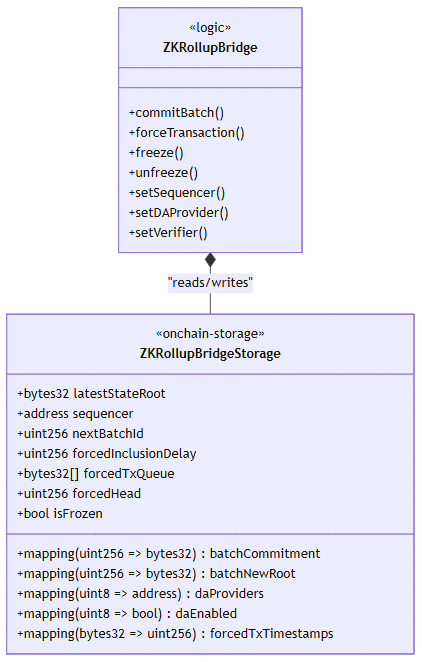
\includegraphics[width=0.95\linewidth]{figures/contract-storage-model.png}
  \caption{Contract Storage Model.}
  \label{fig:contract-storage}
 \end{adjustwidth}
\end{figure}

As illustrated in Figure~\ref{fig:contract-storage}, the storage layout includes the current \texttt{latestStateRoot}, batch commitment mappings, and configuration mappings for DA providers. This state is sufficient to support deterministic state progression and verifiable linkage between submitted batch commitments and the accepted rollup head.

\subsubsubsection{Censorship Resistance and Lifecycle}

The bridge incorporates a censorship-resistance mechanism that constrains sequencer behavior using an explicit lifecycle.

\begin{figure}[htbp]
 \begin{adjustwidth}{0cm}{}
  \centering
  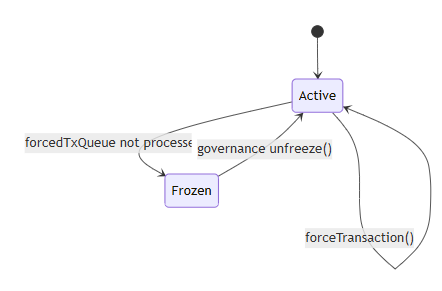
\includegraphics[width=0.95\linewidth]{figures/contact-state-daigram-lifecycle.png}
  \caption{Contract Lifecycle and Censorship Resistance.}
  \label{fig:contract-lifecycle}
 \end{adjustwidth}
\end{figure}

Through \texttt{forceTransaction}, users can enqueue transactions directly on L1. If the sequencer does not process forced transactions within \texttt{forcedInclusionDelay}, the bridge transitions from \textbf{Active} to \textbf{Frozen} (Figure~\ref{fig:contract-lifecycle}). In the Frozen state, normal batch commitments are halted, signaling that the centralized sequencer is not honoring the escape hatch guarantees. This mechanism protects users by preventing silent continuation under censorship assumptions and creates a clear safety boundary until governance action is taken or a mass-exit path (future work) is invoked.

\begin{lstlisting}[style=rustStyle, caption={Forced Transaction Mechanism}, label={lst:force-tx}]
function forceTransaction(bytes32 _txHash) external {
    if (isFrozen) revert BridgeFrozenError();

    // Set deadline for inclusion
    uint256 deadline = block.number + forcedInclusionDelay;
    forcedTxTimestamps[_txHash] = deadline;
    forcedTxQueue.push(_txHash);

    emit ForcedTransactionEnqueued(_txHash, deadline);
}
\end{lstlisting}

\subsubsubsection{DA Providers}

DA verification is abstracted behind the \texttt{IDAProvider} interface, enabling different validation logic depending on the chosen DA mode:

\begin{lstlisting}[style=rustStyle, caption={IDAProvider Interface}, label={lst:ida-provider}]
interface IDAProvider {
    function computeCommitment(
        bytes calldata batchData,
        bytes calldata daMeta
    ) external view returns (bytes32);

    function validateDA(bytes32 commitment, bytes calldata daMeta) external view;

    function mode() external pure returns (uint8);
}
\end{lstlisting}

\begin{itemize}
    \item \textbf{CalldataDA}: validates that the required batch data is present in the transaction payload.
    \item \textbf{BlobDA}: verifies \texttt{blobhash} against the expected commitment, ensuring the blob data matches the submission.
    \item \textbf{OffChainDA}: accepts a commitment (or pointer such as a CID) and delegates availability guarantees to an external data layer.
\end{itemize}

The \textbf{BlobDA} implementation (for EIP-4844) validates that the commitment matches the versioned hash of the attached blob, ensuring that the data is available on the consensus layer.

\begin{lstlisting}[style=rustStyle, caption={BlobDA Implementation}, label={lst:blob-da}]
contract BlobDA is IDAProvider {
    function validateDA(bytes32 commitment, bytes calldata daMeta) external view override {
        (bytes32 expectedVersionedHash, uint8 blobIndex) = abi.decode(daMeta, (bytes32, uint8));

        // 1. Check consistency
        if (commitment != expectedVersionedHash) revert InvalidCommitment();

        // 2. Verify against EVM intrinsic blobhash opcode
        bytes32 actual = blobhash(blobIndex);
        if (actual == bytes32(0)) revert NoBlobAttached();
        if (actual != expectedVersionedHash) revert BlobHashMismatch();
    }
}
\end{lstlisting}

\subsubsection{Verification Sequence}

\begin{figure}[htbp]
 \begin{adjustwidth}{0cm}{}
  \centering
  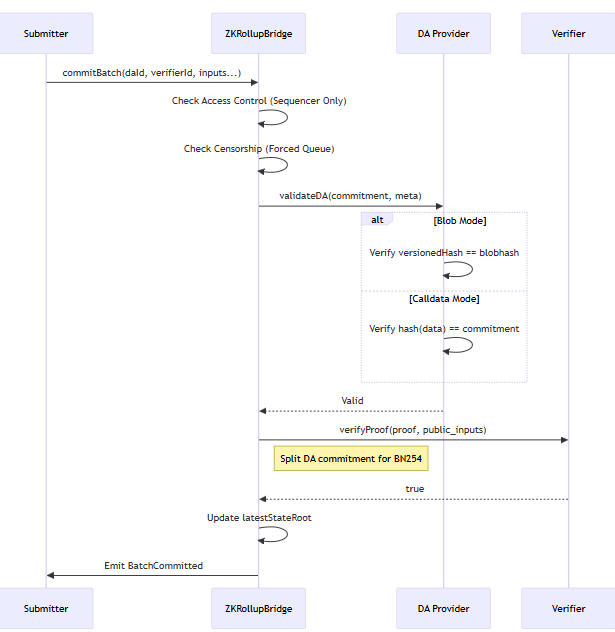
\includegraphics[width=0.95\linewidth]{figures/on-chain-verification-sequnce.png}
  \caption{On-Chain Verification Sequence.}
  \label{fig:contract-verification}
 \end{adjustwidth}
\end{figure}

When the Submitter calls \texttt{commitBatch}, the bridge executes a strict sequence of checks to ensure correctness and safety (Figure~\ref{fig:contract-verification}):
\begin{enumerate}
    \item \textbf{Access Control}: verifies that the caller is the authorized sequencer address.
    \item \textbf{Censorship Check}: verifies that forced transactions have not exceeded the allowed delay window.
    \item \textbf{DA Validation}: invokes the configured \texttt{IDAProvider} to validate the DA commitment (e.g., blobhash or calldata-derived hash).
    \item \textbf{Proof Verification}: invokes the selected \texttt{IVerifier} to verify the proof against public inputs (old root, new root, DA commitment chunks).
    \item \textbf{State Update}: updates \texttt{latestStateRoot} and emits \texttt{BatchCommitted} if all checks succeed.
\end{enumerate}

\subsubsection{Design Rationale and Trade-offs}

\paragraph{Modular Verification}
Decoupling the proof verification logic from the bridge (via the \texttt{IVerifier} interface) allows for upgrading the proof system without redeploying the main bridge contract. This is essential for a research testbed where cryptographic primitives are subject to change.

\paragraph{Censorship Resistance via Forced Transactions}
The \texttt{forceTransaction} mechanism (Listing~\ref{lst:force-tx}) introduces a trade-off: it adds complexity and potential state bloat (tracking the forced queue) but provides a fundamental security guarantee. Without it, the centralized sequencer could effectively freeze user funds. The use of a time-delayed trigger (\texttt{forcedInclusionDelay}) balances this by giving the sequencer a grace period to process legitimate transactions before the "freeze" mode is activated.

\paragraph{EIP-4844 Blob Integration}
Adopting EIP-4844 (Listing~\ref{lst:blob-da}) requires the contract to verify ephemeral data commitments (`blobhash`) rather than permanent calldata. This significantly reduces gas costs but requires the ecosystem (indexers, explorers) to support blob data retrieval, as it is pruned from L1 nodes after approx. 18 days.

\subsubsection{Current Limitations}

The current contract layer is fully functional for benchmarking and controlled experimentation, but it has known PoC limitations:
\begin{itemize}
    \item \textbf{Deposit Functionality}: \texttt{ZKRollupBridge.sol} does not currently implement a native \texttt{deposit} function for bridging assets from L1 to L2. Initial funding is handled via genesis allocation or sequencer-privileged minting in \texttt{dev\_mode}.
    \item \textbf{Proof Aggregation}: verification is executed per batch. Aggregating multiple batch proofs into a single L1 verification step—an important optimization for production cost reduction—is not yet implemented.
\end{itemize}
